\section{Théorie} \label{sec: theory}
    Les attracteurs sont des structures fondamentales en théorie du chaos qui
    jouent un rôle clé dans la compréhension du comportement chaotique des
    systèmes. Dans cette section, nous allons explorer en détail le concept
    d'attracteur en théorie du chaos, en examinant les propriétés mathématiques
    qui les caractérisent.

\subsection{Attracteurs} \label{subsec: attractors}
    Pour un système dynamique dissipatif donné, l'attracteur est définit par
    un sous-ensemble d'états dans l'espace des phases vers lesquels la
    solution au système converge si les conditions initiales de ladite solution
    sont comprises dans le bassin d'attraction de l'attracteur. Ici, le
    \textit{bassin d'attraction} représente une zone de l'espace des phases
    dont les conditions initiales mènent à des trajectoires qui convergent vers
    un attracteur. Mathématiquement, on dit que le bassin d'attraction $W$
    d'un attracteur $A$ est
    \begin{align}
        W(A) = \{r\in R\;\;|\;\lim_{t\to\infty} f(r, t)\in A\},
    \end{align}

    où ici $r$ représente un ensemble de condition initiales appartenant à
    l'espace des phases $R$ et $f(r, t)$ la trajectoire de la solution.
    Autrement-dit, l'attracteur est un sous-ensemble de solutions qui permet
    d'identifier et de prédire une tendance globale dans la trajectoire d'une
    solution donnée d'un système chaotique, et ce, malgré sa nature
    imprévisible. \\

    L'attracteur de Lorenz que l'on nommera ici $L$ est l'un des exemples les
    plus célèbres d'un attracteur chaotique dans la théorie des systèmes
    dynamiques \cite{lorenz}. Cet attracteur est le fruit d'un système
    dynamique non linéaire à trois dimensions qui décrit le comportement d'un
    fluide en mouvement. Mathématiquement, l'attracteur de Lorenz est défini
    par un ensemble d'équations différentielles ordinaires, qui décrivent
    l'évolution de trois variables dynamiques $(x, y, z)$ en fonction du temps
    et des paramètres $\sigma, \rho$ et $\beta$ qui régissent le comportement
    du système
    \begin{align}
        L = \left\{
        \begin{array}{c}
           \Dot{x} = \sigma(y - x) \\
           \Dot{y} = x(\rho - z) - y \\
           \Dot{z} = xy - \beta z,
        \end{array}
        \right.
        \label{eq : lorenz}
    \end{align}

    où les paramètres $\sigma, \rho$ et $\beta$ sont respectivement le nombre
    de Prandtl, le nombre de Rayleigh et un coefficient géométrique quelconque.
    Un second attracteur initialement proposé par Otto Rössler en 1976 est
    l'attracteur de Rössler \cite{rossler}. Celui-ci possède une forme
    particulière et n'a qu'une seule de ses trois équations qui possède un
    terme non linéaire
    \begin{align}
        R = \left\{
        \begin{array}{c}
           \Dot{x} = -y - z \\
           \Dot{y} = x + ay \\
           \Dot{z} = b + z(x - c),
        \end{array}
        \right.
        \label{eq : rossler}
    \end{align}

    avec $a, b$ et $c$ des paramètres numériques qui régissent le comportement
    du système. Le dernier attracteur que nous allons étudier est celui
    introduit par Bouali en 2013, qui est non seulement par définition très
    sensible aux conditions initiales, mais également à la source du phénomène
    unique de chevauchement d'attracteurs \cite{bouali}. Les équations
    différentielles non-linéaires qui décrivent cet attracteur sont
        \begin{align}
        B = \left\{
        \begin{array}{c}
           \Dot{x} = \alpha x(1 - y) - \beta z \\
           \Dot{y} = -\gamma y(1 - x^2) \\
           \Dot{z} = \mu x,
        \end{array}
        \right.
        \label{eq : bouali}
    \end{align}

    où les paramètres $\alpha, \beta, \gamma$ et $\mu$ sont une fois de plus
    des coefficients numériques responsables du comportement de l'attracteur.

\subsection{Exposants de Lyapunov} \label{subsec: lyapunov}
    Nous avons définit que les systèmes dynamiques dissipatifs sensibles au
    changement infinitésimal des conditions initiales sont chaotiques et donc
    que deux trajectoires peuvent se voir diverger rapidement. Soit deux
    positions initiales de l'espace des phases $\bm{x}(t)$ et $\bm{x}(t) +
    \bm{\delta}_0$ tels que montrés sur la figure \ref{fig: theo_lyapunov}
    \begin{figure}[h!]
        \centering
        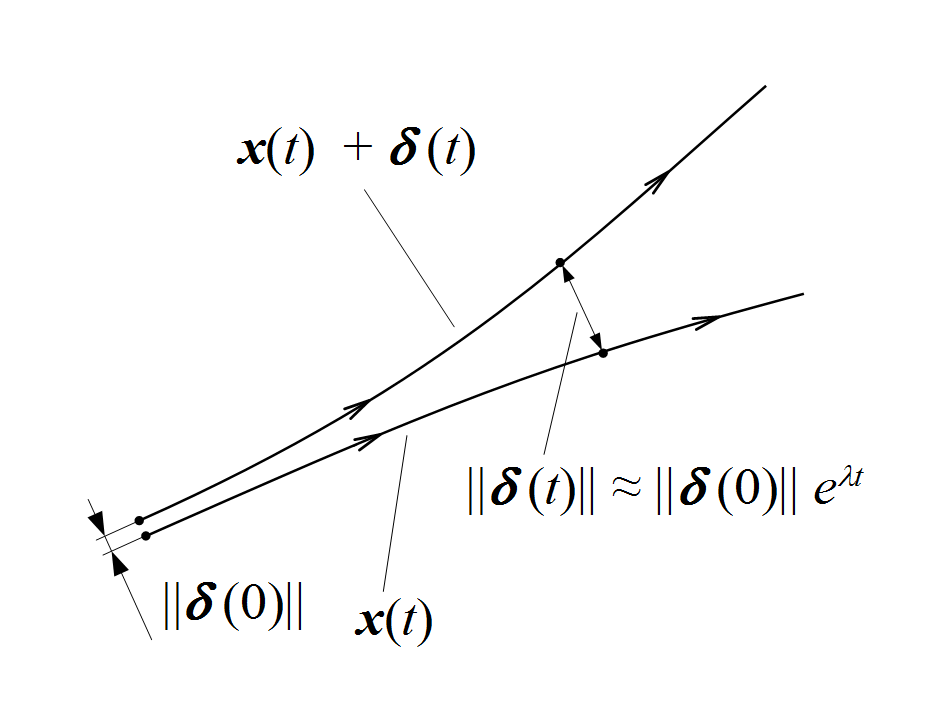
\includegraphics[scale=0.3]{figs/Orbital_instability_(Lyapunov_exponent).png}
        \caption{Schéma qui exprime l'évolution de la distance entre deux
        trajectoires $|\bm{\delta}(t)|$ initialement espacées d'un déplacement
    infinitésimal $|\bm{\delta_0}|$ en fonction du temps \cite{LEs_wiki}.}
        \label{fig: theo_lyapunov}
    \end{figure}

    on considère qu'au temps $t=0$ ces trajectoires ont été éloignées du
    vecteur déplacement $\bm{\delta}_0$ tel que sa norme $|\bm{\delta}_0|$ soit
    infinitésimale. Dans le contexte de systèmes chaotique, on trouve qu'après
    un temps d'évolution $t$, la norme du déplacement entre les trajectoires
    est donné par
    \begin{align}
        |\bm{\delta}(t)| \simeq |\bm{\delta}_0|e^{\lambda t},
        \label{eq : lyapunov_delta}
    \end{align}

    où l'on appelle la quantité $\lambda$ \textit{l'exposant de Lyapunov}. On
    accède à cette quantité avec quelques manipulation
    \begin{align}
        \lambda \simeq
        \frac{1}{t}\ln\qty[\frac{|\bm{\delta}(t)|}{|\bm{\delta}_0|}],
    \end{align}

    où pour un système avec pas temporels discrets tels que l'itération
    $x_{n + 1} = f(x_n)$, se traduit par
    \begin{align}
        \lambda(x_0) = \lim_{n\to\infty}\sum_{i = 0}^{n - 1}\ln(f'(x_i)),
    \end{align}

    avec $x_0$ le point qui correspond à la condition initiale. On voit ici
    que pour des solutions calculées à l'aide d'algorithmes, il est possible
    de remplacer la limite itérative infinie par un algorithme de convergence
    judicieusement choisi tel que \textit{l'algorithme epsilon}. Il est
    cependant important de noter que jusqu'ici, nous n'avons introduit qu'un
    seul exposant $\lambda$ (le plus élevé conventionnellement), mais un
    système de dimension $N$ possède naturellement $N$ exposants de Lyapunov.
    On appelle ces valeurs le \textit{spectre de Lyapunov} d'un système. Ce
    spectre possède plusieurs propriétés intéressantes pour l'analyse des
    systèmes dynamiques \cite{LEs}: \\
    \begin{itemize}
        \item[$\diamond$] Les composantes du spectres sont indépendantes du
            métrique utilisé pour leur calcul ainsi que du choix des variables.
            Cela permet de conclure sur l'objectivité et la pertinence du
            spectre de Lyapunov. \\
        \item[$\diamond$] Si l'exposant le plus élevé du spectre est positif
            témoigne généralement d'instabilités exponentiellement importantes
            et consitue une définition de ce que l'on pourrait appeler chaos. \\
        \item[$\diamond$] La somme du spectre de Lyapunov permet de mesurer
            le taux contraction des volumes de l'espace des phases. Pour des
            systèmes dissipatifs, une somme $\sum_i\lambda_i < 0$ signifie que
            les volumes décroissent exponentiellement à 0 alors qu'une somme
            nulle implique la conservation des volumes de l'espace des phases.
    \end{itemize}
